\chapter{Production autonome d’énergie pour site isolé}


\textit{Nota : Les dispositifs et dimensionnements présentés ci-après constituent une approche simplifiée du problème.}

Le cadre est celui d’un site isolé, que l’on souhaite alimenter à partir de panneaux photovoltaïques (PV) et batteries de stockage.

Le site consomme de l’énergie en permanence avec une puissance ``talon'' et des pointes de consommations au cours de la journée. 

Pour maintenir un fonctionnement durant la nuit, un stockage d’énergie par batteries est associé aux PV.

La fourniture d’énergie est faite en courant alternatif, la tension de service de 230 VAC – 50 Hz étant générée au moyen d’un onduleur monophasé.

L’architecture générale du dispositif est ainsi la suivante :

\begin{figure}[h]
\centering
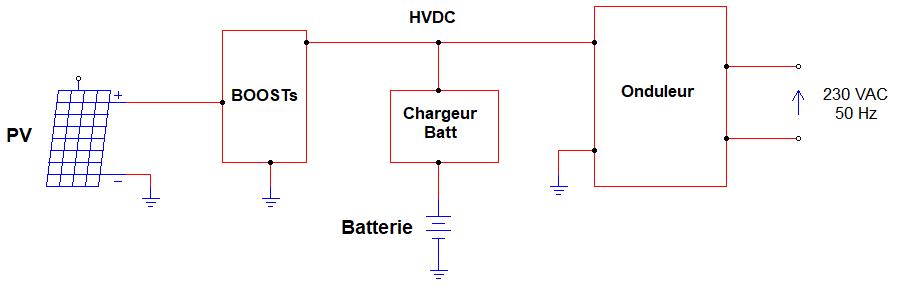
\includegraphics[width=0.8\linewidth]{TD_Boost_2Q_Onduleur/fig/Archi_Globale.png}
\caption{Architecture globale}
\end{figure}

\textbf{Données principales}

\underline{Installation :}
\begin{itemize}
\item Puissance talon de l’installation : 300 W
\item Pointes de puissance consommée : 1500 W
\item Durée des pointes de puissance : 3*30 mn entre 11h00 et 15h00.
\end{itemize}

\underline{PV :}
\begin{itemize}
\item Les PV sont orientés au sud, avec une inclinaison de $35^\circ$ . L’installation se trouve dans les Alpes, au sud de Briançon, dans une zone géographique où l’irradiation moyenne annuelle est de $1500\ kWh/m^2$ (en tenant compte des ombrages portés).

\item La data sheet d’un PV donne les informations suivantes :
\clearpage
\begin{centering}
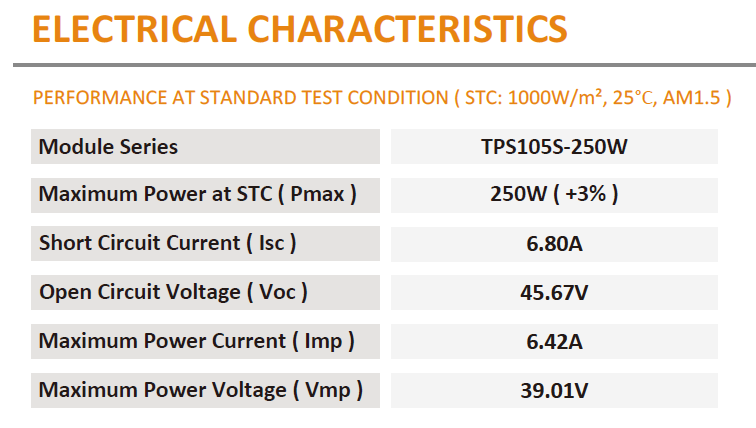
\includegraphics[width=0.49\linewidth]{TD_Boost_2Q_Onduleur/fig/elec_specif.png}
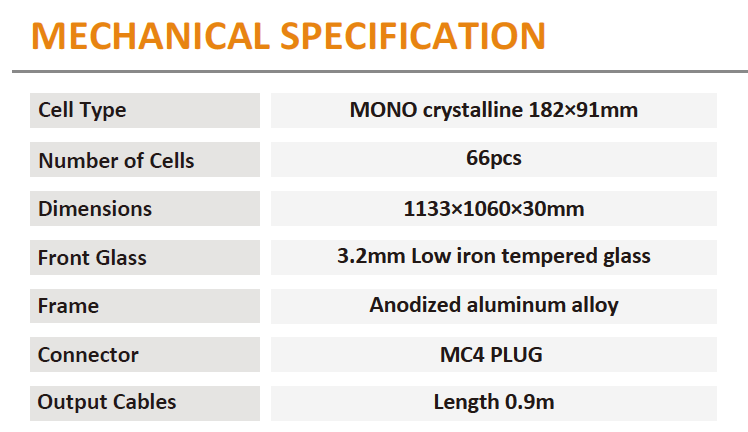
\includegraphics[width=0.49\linewidth]{TD_Boost_2Q_Onduleur/fig/meca_specif.png}
\end{centering}


\item Le rendement global des PV est de 20 \% (tenant compte du ratio\newline [surface cellules / surface totale] et on considère que le rendement global de la chaîne de conversion d’énergie est de 90 \% (cumul de convertisseurs, pertes en lignes, …).
\end{itemize}



\section*{Préliminaires}
Déterminer :
\begin{enumerate}
\item L’énergie consommée par l’installation par jour et sur une année.
\item La surface nécessaire de PV pour permettre l’alimentation du dispositif en tenant compte des rendements.
\item Le nombre minimum de PV nécessaires.
\end{enumerate}


\section{Convertisseurs BOOST}
\label{sec:Convertisseur_BOOST}

On décide d’implanter \textbf{12 PV}, associés en deux groupes de PV en série. Chaque groupe de PV est connecté à une entrée d’un convertisseur DC-DC de type BOOST.
Ainsi, la structure développée du ``BOOST'' de la figure 1 est la suivante :

\begin{figure}[h]
\centering
\includegraphics[width=0.6\linewidth]{TD_Boost_2Q_Onduleur/fig/Archi_Boost.png}
\caption{Architecture Boost}
\end{figure}

On suppose que tous les PV sont éclairés de façon uniforme de sorte que chaque groupe de PV fourni la moitié de la puissance instantanée consommée.

La tension de sortie HVDC est asservie à \textbf{500 V} par des boucles de régulation agissant sur les rapports cycliques des transistors Q1 et Q2.

La fréquence de découpage de Q1 et Q2 est fixe et égale à \textbf{Fd = 50 kHz}.

\underline{On ne s’intéresse pour l’instant qu’au BOOST 1 et on suppose que tous les composants}\newline
\underline{sont parfaits.}

En considérant que :
\begin{itemize}
\item la tension d’entrée du BOOST (sur C1) et HVDC sont rigoureusement constantes sur une période de découpage
\item l’ondulation de courant c-à-c $\Delta I$ dans L1 représentent 20 \% du courant moyen d’entrée.
\item On se place dans un régime de conduction continue.
\end{itemize}

\begin{enumerate}
\item Représenter les courants dans L1, Q1 et D1 ainsi que les tensions à leurs bornes, sur deux périodes de découpage et pour un rapport cyclique de 50 \%.

\item Déterminer l’expression de HVDC en fonction de la tension d’entrée, notée Vpv, et du rapport cyclique $\alpha$.
De même, exprimer la relation entre le courant Ipv (courant moyen dans L1) et le courant de sortie $I_{HVDC}$.

\item Déterminer littéralement :
\begin{enumerate}
\item La tension maximale appliquée aux bornes de Q1 et D1.
\item Les valeurs moyennes et maximales des courants dans L1, Q1 et D1 en fonction de Ipv, $\Delta I$ et du rapport cyclique.
\item Résumer ces résultats dans un tableau de contraintes (utile pour le choix des composants).
\end{enumerate}

On considère maintenant les deux BOOST en fonctionnement et se répartissant la puissance de façon égale. Les commandes de Q1 et Q2 sont synchrones.
Les conditions d’environnement sont les conditions STC ($1000 W/m^2$ - $25^\circ C$).

On considère également une séquence de fonctionnement durant laquelle (1er cas extrême) :
\begin{itemize}
\item la puissance consommée par la charge est maximale
\item la batterie n’est pas totalement chargée et consomme le différentiel de puissance entre la puissance consommée par la charge et la puissance fournie par les PV, qui correspond à la `` puissance crête'' totale.
\end{itemize}

\item Déterminer :
\begin{enumerate}
\item La puissance totale $P_{cT}$ que peuvent fournir les PV compte tenu de l’irradiation.
\item La puissance qui transite dans chaque BOOST.
\item La puissance consommée par la batterie.
\end{enumerate}

\item Dans ces conditions de fonctionnement, pour chacun des deux BOOST déterminer :
\begin{enumerate}
\item La tension d’entrée Vpv.
\item Le courant d’entrée Ipv.
\item Le rapport cyclique de commande des transistors.
\item La valeur de L pour que $\Delta I$ représente 20 \% de Ipv.
\item Les contraintes appliquées sur les composants de puissance Q et D (tension max., courant moyen et max.) 
\end{enumerate}

On considère maintenant que la puissance consommée par la charge est la puissance minimale et que la batterie est totalement chargée (2nd cas extrême).

\item On suppose que les conditions sont toujours STC et que la tension de sortie d’un PV est de 44 V.
\begin{enumerate}
\item Déterminer la puissance fournie par chaque groupe de PV et le courant d’entrée de chaque BOOST.
\item Les BOOST fonctionnent-ils toujours en régime de conduction continue ?
\item Représenter le courant d’entrée dans L ainsi que la tension à ses bornes.
\item Exprimer le courant d’entrée Ipv en fonction de Vpv, HVDC, L, Fd et le temps de conduction du transistor $t_{on}$.
\item Déterminer la nouvelle valeur de rapport cyclique permettant de maintenir HVDC à 500 V.
\end{enumerate}

\end{enumerate}

\newpage
\section{Chargeur de Batterie (Half-Bridge)}

Pour permettre une alimentation en électricité durant la nuit, un pack de batteries est mis en place.

La structure de puissance associée aux batteries est celle d’un convertisseur réversible de type ``Half Bridge'' (Hacheur 2 quadrants). Ce convertisseur permet d’alimenter l’installation à partir du pack durant la nuit, et de recharger le pack à partir des PV pendant la journée.

\vspace{0.5cm}
Le schéma suivant présente cette structure :

 \begin{figure}[h]
\centering
\includegraphics[width=0.8\linewidth]{TD_Boost_2Q_Onduleur/fig/Archi_2Q.png}
\caption{Architecture hacheur 2 quadrants}
\end{figure}


Dans tous les cas, les boucles de régulation des BOOST et du Half-Bridge permettent de maintenir \textbf{HVDC = 500 V.}

La tension du pack batterie est supposée constante et égale à \textbf{Ubatt = 120 V} (38 éléments de 3.2 V / Technologie LiFePo4).

Une boucle de limitation du courant batterie incluse dans le BMS (Battery Management System) limite celui-ci à $I_{batt\_max} = 10\ A$.

Les transistors Q3 et Q4 sont pilotés en commandes complémentaires à une fréquence fixe de 50 kHz. Les temps morts sont négligés.

Par la suite, le rapport cyclique désigne le rapport du temps de conduction de Q3 ramené à la période de découpage.

\begin{enumerate}
\item Pour un rapport cyclique donné (0.3 par exemple) et en régime de conduction continue, représenter, pour des courants de charge ($I_{L3} > 0$) et de décharge de la batterie de mêmes valeurs absolues :
\begin{enumerate}
\item Les courants dans L3, Q3 et Q4.
\item La tension aux bornes de L3.
\item Présenter les sens de circulation du courant dans L3.
\end{enumerate}

\item Exprimer la relation entre la tension batterie et HVDC en fonction du rapport cyclique de commande de Q3 noté $\alpha_{HB}$ (en régime de conduction continue).

Dans un premier temps, on se place en journée pendant que le pack se recharge dans une configuration correspondante à la question 4 du TD \ref{sec:Convertisseur_BOOST}. Dans cette configuration, le courant de charge de la batterie est $I_{batt\_max}$.

\item Le convertisseur Half Bridge fonctionne-t-il en ``Buck'' ou en ``Boost'' ? A quoi sert C3 ?

\item On souhaite que l’ondulation de courant dans L3 représente 30 \% de son courant moyen (soit 3 A). Déterminer :

\begin{enumerate}
\item Le rapport cyclique de commande de Q3
\item La valeur à donner à L3
\end{enumerate}

\item Pour ce point de fonctionnement, déterminer les contraintes en tension, courant maximum et courant moyen sur Q3 et Q4.

On se place toujours durant la journée, mais maintenant dans une configuration où l’installation appelle sa puissance maximale (1800 W). Les conditions météorologiques sont telles que les PV ne peuvent fournir que 1000 W (rendement des Boost compris).

\item Quelle est la puissance fournie par la batterie et que vaut son courant ?

\item Le fonctionnement du HB est-il ``Buck'' ou ``Boost'' ?

\item Que vaut le rapport cyclique de commande de Q3 ?  Le convertisseur HB fonctionne-t-il toujours en régime de conduction continue ? Représenter les courants dans L3, Q3 et Q4 et la tension $V_{L3}$ en précisant les valeurs numériques remarquables. Donner les schémas équivalents aux deux phases de fonctionnement en précisant les sens de circulation des courants.

\item La nuit, la batterie fournie seule l’énergie à l’installation et la puissance consommée est de 300 W. On suppose que le rendement du HB est unitaire.
\begin{enumerate}
\item Déterminer la valeur du rapport cyclique de Q3 pour maintenir HVDC à 500 V
\item Représenter le courant dans L3 en précisant sa valeur moyenne.
\end{enumerate}

\item En tenant compte d’un rendement global du [HB + Onduleur] de 90 \%, quelle doit être la capacité minimale (en Ah) du pack pour maintenir une autonomie durant 16h00 d’affilée et avec un taux de décharge maximum de 90 \% (sur cette période, les phases à puissance maximale n’apparaissent pas).

\end{enumerate}

\newpage
\section{Onduleur monophasé MLI sur charge RL}

On s'intéresse maintenant à l'onduleur monophasé. Le réseau est modélisé par une charge R-L série. Le schéma de principe est le suivant :

\begin{figure}[h]
\centering
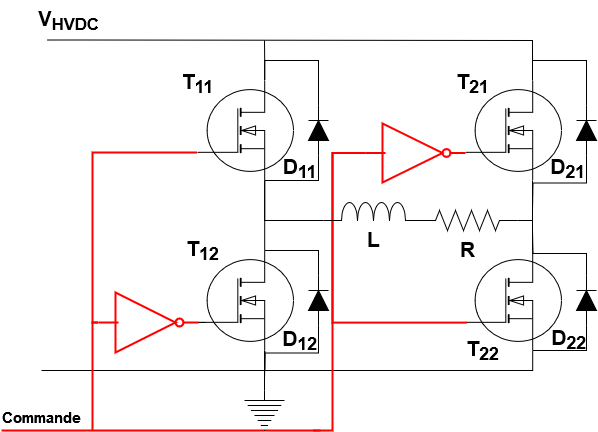
\includegraphics[width=0.8\linewidth]{TD_Boost_2Q_Onduleur/fig/Onduleur.png}
\end{figure}

\begin{itemize}
\setlength\itemsep{-1mm}
\item Les transistors fonctionnent en MLI à une fréquence de découpage $F_d$ très grande devant la fréquence de la tension à reconstituer en sortie.
\item Le rapport cyclique est variable dans le temps et sera noté : $\alpha(t) = 0.5 + \delta_\alpha sin(\omega .t)$.
\end{itemize}



Par la suite, on désigne par :

\begin{itemize}
\setlength\itemsep{-1mm}
\item $V_0$ : la tension aux bornes de l’ensemble $L - R$ (tension de sortie de l’onduleur).
\item $I_R$ : le courant dans la charge $R - L$
\end{itemize}

Les principales caractéristiques de la charge sont :

\begin{itemize}
\setlength\itemsep{-1mm}
\item Schéma équivalent : $R - L$ série, avec $L = 30 mH$
\item Puissance nominale : 1500 W
\item Tension nominale aux bornes de $R$ : $U_{Rn} = 230 V$ (valeur efficace)
%\item Après la mise sous tension, la puissance absorbée par la charge évolue linéairement de 300 à 500 W pendant 300 secondes, puis se stabilise à 500 W.
%\item Dans le même intervalle de temps, la tension efficace aux bornes de $R$ (notée : $U_R$), évolue linéairement de 40 à 100 V.
\end{itemize}

\begin{enumerate}
%\item Sur un même graphe, et durant les 400 secondes suivant la mise sous tension, représenter les évolutions :
%
%\begin{enumerate}
%\item de la puissance absorbée par la charge
%\item de la tension aux bornes de $R$ : $U_R$
%\item du courant efficace dans la charge $I_R$
%\end{enumerate}

\item Tension de sortie $V_0$

\begin{enumerate}
\item Représenter l’allure de la tension de sortie pour un rapport cyclique $\alpha > 0.5$ et sur une période de découpage
\item Exprimer la valeur moyenne de $V_o$ sur une période de découpage en fonction du rapport cyclique $\alpha$ et de $V_{DC}$
\item Exprimer l'évolution temporelle de la valeur moyenne (sur une période de découpage) de la tension de sortie \hbox{$<V_0>(t)$} en fonction de $V_{DC}$ et $\delta_\alpha$
\item Déterminer la valeur efficace de $<V_0>(t)$ (notée $V_{0\ eff}$) en fonction de $V_{HVDC}$ et $\delta_\alpha$
\item En négligeant la composante de courant due au découpage, donner l’expression du courant dans $R$ ($I_R(t)$) en prenant $<V_0>(t)$ en référence de phase
\item Exprimer la valeur efficace du courant dans $R$ en fonction de $V_{0\ eff}$, $R$, $L$ et $\omega$
\item Exprimer le déphasage $\varphi$ entre $I_R(t)$ et $<V_0>(t)$ en fonction de $R$, $L$ et $\omega$
\item Exprimer le facteur de puissance de la charge $RL$ en fonction de $R$, $L$ et $\omega$
\item Exprimer la puissance dans $R$ en fonction de $\delta_\alpha$, $V_{HVDC}$, $R$, et $\varphi$.
\end{enumerate}
\item Fonctionnement à puissance nominale (1500W).

Pour rappel, la tension d’alimentation $V_{HVDC}$ est la tension du bus continu, $V_{HVDC}=500 V$. La fréquence de la tension reconstituée ($<V_0>(t)$) est de \textbf{50 Hz}.

\begin{enumerate}
\item Déterminer la valeur de $R$ pour ce point de fonctionnement
\item Déterminer la valeur du facteur de puissance
\item Etablir le diagramme de Fresnel liant $V_0$, $I_R$ et $U_R$
\item Déterminer la valeur de la tension aux bornes de $L$
\item Déterminer la valeur à donner à $V_{0\ eff}$
\item Déterminer la valeur à donner à $\delta_\alpha$ pour obtenir ce point de fonctionnement
%\item Déterminer les variations possibles de $\delta_\alpha$ compte tenu des variations possibles de la valeur efficace de la tension réseau (pour maintenir le point de fonctionnement nominal)
%\item En gardant la valeur de $R$, déterminer la puissance maximale transférable dans $R$ pour une tension réseau de 230 V efficace
\end{enumerate}

%\item Lors du démarrage (à la mise sous tension) quand la tension réseau est à son nominal (230 V), déterminer :
%
%\begin{enumerate}
%\item le facteur de puissance
%\item la valeur à donner à $V_0$ (valeur efficace)
%\item l’expression du rapport cyclique
%\end{enumerate}

\item Déterminer la tension maximale à l’état bloqué et le courant maximum pour chaque interrupteur de l’onduleur (la composante de courant à la fréquence de découpage est toujours négligée)
\end{enumerate}